\begin{pastexam}[label={px:df3-099-ds-03}]{地方三等資訊處理 99 年 第三題}
（申論；15 分）

考慮某地區的地圖，地圖上有 $n$ 個城市，城市之間共有 $m$ 條相通的公路，每條公路有一個長度（例如，10 公里）。某人經常需從城市 $S$ 出發，開車前往另一城市 $T$ 送貨，請你設計一個軟體系統的資料結構與演算法，幫忙找出路程最短的建議路徑與該路徑的總長度。（每小題 5 分，共 15 分）
\begin{itemize}[leftmargin=2.2em]
\item[㈠] 請設計一資料結構表示出地圖之 $n$ 個城市、$m$ 條公路及公路長度。
\item[㈡] 依據你設計的資料結構，寫出 Dijkstra 演算法，找出路程最短的建議路徑與該路徑的總長度，並舉例說明。
\item[㈢] 分析 Dijkstra 的時間複雜度。
\end{itemize}
\end{pastexam}

\begin{pastsoln}
公路是雙向的，地圖是\textbf{無向加權圖}，長度都是正數，正好適用 Dijkstra（資結書第~25.2~節）。 城市編號 $1..n$。

\textbf{㈠ 資料結構}。 用\textbf{鄰接串列}（資結書第~21.2~節）：陣列 $\mathit{adj}[1..n]$，$\mathit{adj}[u]$ 是一條鏈結串列，
每個串列節點存三欄 $(v, \mathit{len}, \mathit{next})$，表示 $u$ 和 $v$ 之間有一條長 $\mathit{len}$ 的公路。 一條公路
$\{u, v\}$ 在 $\mathit{adj}[u]$ 和 $\mathit{adj}[v]$ 各存一次，共 $2m$ 個串列節點，空間 $\Theta(n + m)$。 （城市之間的公路
通常遠少於 $n^2$ 條，鄰接串列比 $n \times n$ 的鄰接矩陣省空間；若圖很密，也可以用矩陣，$\mathit{len}[u][v] = \infty$
表示沒有公路。）

另外準備三個陣列：$\mathit{dist}[v]$ 是目前已知 $S$ 到 $v$ 的最短距離，$\mathit{prev}[v]$ 是那條路徑上 $v$ 的前一個城市
（用來還原路徑），$\mathit{done}[v]$ 表示 $v$ 的最短距離是否已經確定。

\textbf{㈡ Dijkstra 演算法}。 每次從還沒確定的城市中，挑 $\mathit{dist}$ 最小的 $u$，宣告它確定，再用 $u$ 的每條公路去更新
（鬆弛）鄰居的距離。 用最小堆積（優先佇列）挑最小值：
\begin{pseudo}[unbreakable]{Dijkstra：$S$ 到各城市的最短距離與前一個城市}
\Procedure{Dijkstra}{$\mathit{adj}, n, S$}
    \For{$v \gets 1$ \To $n$}
        \State $\mathit{dist}[v] \gets \infty$；$\mathit{prev}[v] \gets 0$；$\mathit{done}[v] \gets \FALSE$
    \EndFor
    \State $\mathit{dist}[S] \gets 0$；$H \gets$ 只有 $(0, S)$ 的最小堆積
    \While{$H$ 不空}
        \State $(d, u) \gets$ \Call{Extract-Min}{$H$}
        \If{$\mathit{done}[u]$}
            \State \textbf{continue} \Comment{過時的項目}
        \EndIf
        \State $\mathit{done}[u] \gets \TRUE$
        \For{$\mathit{adj}[u]$ 上的每個 $(v, \mathit{len})$}
            \If{$\mathit{dist}[u] + \mathit{len} < \mathit{dist}[v]$}
                \State $\mathit{dist}[v] \gets \mathit{dist}[u] + \mathit{len}$；$\mathit{prev}[v] \gets u$
                \State \Call{Insert}{$H, (\mathit{dist}[v], v)$}
            \EndIf
        \EndFor
    \EndWhile
\EndProcedure
\end{pseudo}
結束後 $\mathit{dist}[T]$ 就是最短路徑的總長度（$\infty$ 表示到不了）。 建議路徑從 $T$ 沿 $\mathit{prev}$ 往回走到 $S$，再倒過來輸出
（例如推進堆疊再彈出）。 若只關心 $T$，第 9 行把 $T$ 標成確定時就可以提早結束。 正確性：長度都非負時，被取出的 $u$ 的
$\mathit{dist}[u]$ 已經是最短距離（資結書定理~25.6）。

\textbf{舉例}。 五個城市 $S, A, B, C, T$，公路：$S$–$A$ $4$、$S$–$B$ $1$、$B$–$A$ $2$、$A$–$C$ $1$、$B$–$C$ $5$、$C$–$T$ $3$、
$A$–$T$ $6$（公里）。
\begin{center}
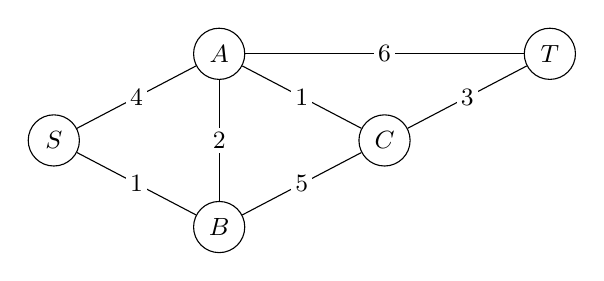
\begin{tikzpicture}[x=1.4cm,y=1.1cm,v/.style={circle,draw,minimum size=6.5mm,inner sep=0pt,font=\small},w/.style={font=\small,fill=white,inner sep=1.5pt}]
\node[v] (S) at (0,0) {$S$};
\node[v] (A) at (1.5,1) {$A$};
\node[v] (B) at (1.5,-1) {$B$};
\node[v] (C) at (3,0) {$C$};
\node[v] (T) at (4.5,1) {$T$};
\draw (S)--node[w]{4}(A); \draw (S)--node[w]{1}(B); \draw (B)--node[w]{2}(A);
\draw (A)--node[w]{1}(C); \draw (B)--node[w]{5}(C); \draw (C)--node[w]{3}(T); \draw (A)--node[w]{6}(T);
\end{tikzpicture}
\end{center}
\begin{center}
\small
\begin{tabular}{lccccc}
\toprule
確定的城市 & $S$ & $A$ & $B$ & $C$ & $T$ \\
\midrule
起始 & $0$ & $\infty$ & $\infty$ & $\infty$ & $\infty$ \\
$S$（0） & \textbf{0} & $4/S$ & $1/S$ & $\infty$ & $\infty$ \\
$B$（1） & & $3/B$ & \textbf{1} & $6/B$ & $\infty$ \\
$A$（3） & & \textbf{3} & & $4/A$ & $9/A$ \\
$C$（4） & & & & \textbf{4} & $7/C$ \\
$T$（7） & & & & & \textbf{7} \\
\bottomrule
\end{tabular}
\end{center}
表中「$d/p$」表示 $\mathit{dist} = d$、$\mathit{prev} = p$，粗體是確定的值。 結果 $\mathit{dist}[T] = 7$；由 $\mathit{prev}$ 往回：
$T \leftarrow C \leftarrow A \leftarrow B \leftarrow S$，建議路徑 $S \to B \to A \to C \to T$，總長 $1 + 2 + 1 + 3 = 7$ 公里。 直接走
$S \to A \to T$ 是 $10$ 公里，比較長。

\textbf{㈢ 時間複雜度}。
\begin{itemize}
\item \textbf{用二元堆積}（上面的寫法）：每條公路在兩端各被看一次，鬆弛共 $2m$ 次，每次成功最多一次 \proc{Insert}；堆積裡
最多 $O(m)$ 個項目，\proc{Extract-Min} 和 \proc{Insert} 各 $O(\log m) = O(\log n)$，共 $O((n + m) \log n)$。
\item \textbf{用陣列找最小值}（不用堆積）：$n$ 次挑最小各掃一遍 $O(n)$，鬆弛共 $O(m)$，合計 $O(n^2 + m) = O(n^2)$；圖很密
（$m$ 接近 $n^2$）時這個版本反而比較好。
\item 用費氏堆積可做到 $O(m + n \log n)$。
\end{itemize}
還原路徑最多走 $n - 1$ 步，$O(n)$，不影響總時間。
\end{pastsoln}
